\documentclass[dvipdfmx]{jsarticle}

\title{ブロック落しゲーム(JavaScript)}
\author{Seiichi Nukayama}
\date{2020-06-21}
\usepackage{tcolorbox}
\usepackage{color}
\usepackage{listings, plistings}

% Java
\lstset{% 
  frame=single,
  backgroundcolor={\color[gray]{.9}},
  stringstyle={\ttfamily \color[rgb]{0,0,1}},
  commentstyle={\itshape \color[cmyk]{1,0,1,0}},
  identifierstyle={\ttfamily}, 
  keywordstyle={\ttfamily \color[cmyk]{0,1,0,0}},
  basicstyle={\ttfamily},
  breaklines=true,
  xleftmargin=0zw,
  xrightmargin=0zw,
  framerule=.2pt,
  columns=[l]{fullflexible},
  numbers=left,
  stepnumber=1,
  numberstyle={\scriptsize},
  numbersep=1em,
  language={Java},
  lineskip=-0.5zw,
  morecomment={[s][{\color[cmyk]{1,0,0,0}}]{/**}{*/}},
}
%\usepackage[dvipdfmx]{graphicx}
\usepackage{url}
\usepackage[dvipdfmx]{hyperref}
\usepackage{amsmath, amssymb}
\usepackage{itembkbx}
\usepackage{eclbkbox}	% required for `\breakbox' (yatex added)
\usepackage{setspace}
\usepackage{multicol}
\fboxrule=1pt
\parindent=1em
\begin{document}

%% 修正時刻: Sun Jun 21 08:35:35 2020


\section{矢印キーでブロックを動かす}

矢印キーでブロックを動かせるようにします。

index.htmlの中に gamekaishi()関数を呼び出しているところが2つあります。
\verb!<body>!タグと\verb!<button>!タグです。
このうち \verb!<body>!タグのほうを変更して、矢印キーの動きに反応するようにします。
以下のように修正してください。

\fbox{\textless onload=''hajime()`` \textbf{onkeydown=''ugokasu(event)``}\textgreater}

引数event で矢印キーの動きを拾い、ugokasu()関数の中に伝えています。

では、ugokasu()関数を書いていきます。

 \begin{lstlisting}[caption=program.js]
  const block = [
  ... (省略) ...
  ];  

  let col;   // blockのx座標 1...10
  let row;   // blockのy座標 0...21

  /**
  * keyCode: 左キー: 37,  上キー: 38,  右キー: 39,  下キー: 40
  */
  function ugokasu(e) {
    const gamegamen = document.getElementById('game');
    const cv = gamegamen.getContext('2d');

    kesu(cv, col, row);

    switch (e.keyCode) {
      case 37:
        col = col - 1;
        break;
      case 38:
        break;
      case 39:
        col = col + 1;
        break;
      case 40:
        break;
    }

    kaku(cv, col, row);
  }
 \end{lstlisting}

 左右キーに反応してブロックが動くようになりました。
 ただ、左右のブロックは突き抜けてしまいますが。

 キーに反応して音を鳴らすようにします。
 kesu() と switch() の間に入れることにします。

 \begin{lstlisting}
  ...(省略)...

  // 音を鳴らす関数(回転音)
  function otoKaiten() {
    document.getElementById('kaiten').play();
  }
  
  /**
  * keyCode: 左キー: 37,  上キー: 38,  右キー: 39,  下キー: 40
  */
  ...(省略)...

  kesu(cv, col, row)

  otoKaiten();         // <=== ここで鳴らす
 \end{lstlisting}

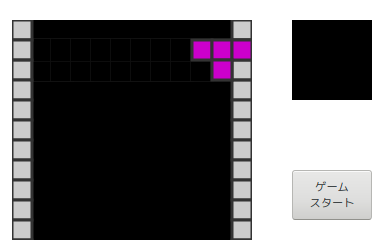
\includegraphics[width=6cm]{game5.png}
 
\end{document}

%% 修正時刻: Sat May  2 15:10:04 2020


%% 修正時刻: Sun Jun 21 11:57:07 2020
